\section*{19. Causal Inference}\label{causal-inference}

In this chapter we discuss causation. Roughly speaking ``\(X\) causes
\(Y\)'' means that changing the value of \(X\) will change the
distribution of \(Y\). When \(X\) causes \(Y\), \(X\) and \(Y\) will be
associated but the reverse is not, in general, true.

We will consider two frameworks for discussing causation. The first uses
notation of \textbf{counterfactual} random variables. The second, used
in the next chapter, uses \textbf{directed acyclic graphs}.

\subsection*{19.1 The Counterfactual Model}\label{the-counterfactual-model}

Suppose that \(X\) is a binary treatment variable where \(X = 1\) means
``treated'' and \(X = 0\) means ``not treated''.

Let \(Y\) be some outcome variable such as the presence or absence of
disease. To distinguish the statement ``\(X\) is associated with \(Y\)''
from the statement ``\(X\) causes \(Y\)'' we need to enrich our
probabilistic vocabulary. We will decompose the response \(Y\) into a
more fine-grained object.

We introduce two new random variables \((C_{0}, C_{1})\) called
\textbf{potential outcomes} with the following interpretation: \(C_{0}\)
is the outcome if the subject is not treated (\(X = 0\)) and \(C_{1}\) is
the outcome if the subject is treated (\(X = 1\)). Then,

\[ Y = \begin{cases}
C_{0} & \text{if } X = 0 \\
C_{1} & \text{if } X = 1
\end{cases}\]

We can express the relationship between \(Y\) and \((C_{0}, C_{1})\) more
succintly by

\[ Y = C_X \]

This equation is called the \textbf{consistency relationship}.

Here is a toy dataset to make the relationship clear:

\[
\begin{array}{cccc}
X & Y & C_{0} & C_{1} \\
\hline
0 & 4 & 4 & * \\
0 & 7 & 7 & * \\
0 & 2 & 2 & * \\
0 & 8 & 8 & * \\
\hline
1 & 3 & * & 3 \\
1 & 5 & * & 5 \\
1 & 8 & * & 8 \\
1 & 9 & * & 9
\end{array}
\]

The asterisks denote unobserved values. When \(X = 0\) we do not observe
\(C_{1}\) in which case we say that \(C_{1}\) is a \textbf{counterfactual}
since it is the outcome you would have had if, counter to the fact, you
had been treated (\(X = 1\)). Similarly, when \(X = 1\) we do not observe
\(C_{0}\) and we say that \(C_{0}\) is counterfactual.

Notice that there are four types of subjects:

\[
\begin{array}{lcc}
\text{Type} & C_{0} & C_{1} \\
\hline
\text{Survivors}       & 1 & 1 \\
\text{Responders}      & 0 & 1 \\
\text{Anti-responders} & 1 & 0 \\
\text{Doomed}          & 0 & 0
\end{array}
\]

Think of all of the potential outcomes \((C_{0}, C_{1})\) as hidden
variables that contain all the relevant information about the subject.

Define the \textbf{average causal effect} or \textbf{average treatment
effect} to be

\[ \theta = \mathbb{E}(C_{1}) - \mathbb{E}(C_{0}) \]

The parameter \(\theta\) has the following interpretation: \(\theta\) is
the mean if everyone were treated (\(X = 1\)) minus the mean if everyone
were not treated (\(X = 0\)). There are other ways of measuring the
causal effect. For example, if \(C_{0}\) and \(C_{1}\) are binary, we define
the \textbf{causal odds ratio}

\[ \frac{\mathbb{P}(C_{1} = 1)}{\mathbb{P}(C_{1} = 0)} \div \frac{\mathbb{P}(C_{0} = 1)}{\mathbb{P}(C_{0} = 0)}\]

and the \textbf{causal relative risk}

\[ \frac{\mathbb{P}(C_{1} = 1)}{\mathbb{P}(C_{0} = 1)} \]

The main ideas will be the same whatever causal effect we use. For
simplicity, we shall work with the average causal effect \(\theta\).

Define the \textbf{association} to be

\[ \alpha = \mathbb{E}(Y | X = 1) - \mathbb{E}(Y | X = 0)\]

Again we could use the odds ratio or other summaries if we wish.

\textbf{Theorem 19.1 (Association is not equal to Causation)}. In
general, \(\theta \neq \alpha\).

\textbf{Theorem 19.3}. Suppose we randomly assign subjects to treatment
and that \(\mathbb{P}(X = 0) > 0\) and \(\mathbb{P}(X = 1) > 0\). Then
\(\alpha = \theta\). Hence, any consistent estimator of \(\alpha\) is a
consistent estimator of \(\theta\). In particular, a consistent
estimator is

\[ \hat{\theta} = \hat{\mathbb{E}}(Y | X = 1) - \hat{\mathbb{E}}(Y | X = 0) = \overline{Y}_{1} - \overline{Y}_{0} \]

is a consistent estimator of \(\theta\), where

\[
\begin{array}{ll}
\hat{Y}_{1} = \frac{1}{n_{1}} \sum_{i: X_{i} = 1} Y_{i}
&
\hat{Y}_{0} = \frac{1}{n_{0}} \sum_{i: X_{i} = 0} Y_{i} \\
n_{1} = \sum_{i=1}^{n} X_{i}
&
n_{0} = \sum_{i=1}^{n} (1 - X_{i})
\end{array}
\]

\textbf{Proof}. Since \(X\) is randomly assigned, \(X\) is independent
of \((C_{0}, C_{1})\). Hence,

\begin{align*}
\theta &= \mathbb{E}(C_{1}) - \mathbb{E}(C_{0}) \\
&= \mathbb{E}(C_{1} | X = 1) - \mathbb{E}(C_{0} | X = 0) \\
&= \mathbb{E}(Y | X = 1) - \mathbb{E}(Y | X = 0) \\
&= \alpha
\end{align*}

The consistency follows from the law of large numbers.

If \(Z\) is a covariate, we define the \textbf{conditional causal
effect} by

\[ \theta_z = \mathbb{E}(C_{1} | Z = z) - \mathbb{E}(C_{0} | Z = z) \]

In a randomized experiment,
\(\theta_z = \mathbb{E}(Y | X = 1, Z = z) - \mathbb{E}(Y | X = 0, Z = z)\)
and we can estimate the conditional causal effect using appropriate
sample averages.

\textbf{Summary}

\begin{itemize}[tightlist]
\item
  Random variables: \((C_{0}, C_{1}, X, Y)\)
\item
  Consistency relationship: \(Y = C_X\)
\item
  Causal Effect: \(\theta = \mathbb{E}(C_{1}) - \mathbb{E}(C_{0})\)
\item
  Association:
  \(\alpha = \mathbb{E}(Y | X = 1) - \mathbb{E}(Y | X = 0)\)
\item
  Random Assignment:
  \((C_{0}, C_{1}) \text{ ⫫ } X \Longrightarrow \theta = \alpha\)
\end{itemize}

\subsection*{19.2 Beyond Binary Treatments}\label{beyond-binary-treatments}

Suppose that \(X \in \mathcal{X}\). The counterfactual vector
\((C_{0}, C_{1})\) now becomes the \textbf{counterfactual process}

\[ \{ C(x) : x \in \mathcal{X} \} \]

where \(C(x)\) is the outcome a subject would have if subjected to
treatment \(x\). The observed response is given by the consistency
relation

\[ Y \equiv C(X) \]

The \textbf{causal regression function} is

\[ \theta(x) = \mathbb{E}(C(x)) \]

The regression function, which measures association, is
\(r(x) = \mathbb{E}(Y | X = x)\).

\textbf{Theorem 19.4}. In general, \(\theta(x) \neq r(x)\). However,
when \(X\) is randomly assigned, \(\theta(x) = r(x)\).

\subsection*{19.3 Observational Studies and Confounding}\label{observational-studies-and-confounding}

A study in which treatment (or exposure) is not randomly assigned is
called an \textbf{observational study}. In these studies, subjects
select their own value of the exposure \(X\). Association and causation
could be quite different. This discrepancy occurs in non-randomized
studies because the potential outcome \(C\) is not independent of
treatment \(X\).

However, suppose we could find groupings of subjects such that, within
each group, \(X\) and \(\{ C(x) : x \in \mathcal{X} \}\) are
independent. This would happen if the subjects are very similar within
groups. For example, suppose we find people who are very similar in age,
gender, educational background and ethnic background. Among those people
we might feel it is reasonable to assume that the choice of \(X\) is
essentially random. These other variables are called \textbf{confounding
variables}. If we denote these variables collectively as \(Z\), then we
can express this idea by saying that

\[ \{ C(x) : x \in \mathcal{X} \} \text{ ⫫ } X | Z\]

If this holds and we observe \(Z\) then we say there is \textbf{no
unmeasured confounding}.

\textbf{Theorem 19.17}. Suppose that $ \{ C(x) : x \in \mathcal{X} \}
\text{ ⫫ } X |{} Z$. Then,

\[ \theta(x) = \int \mathbb{E}(Y | X = x, Z = z) d F_Z(z) dz \]

If \(\hat{r}(x, z)\) is a consistent estimate of the regression function
\(\mathbb{E}(Y | X = x, Z = z)\), then a consistent estimate of
\(\theta(x)\) is

\[ \hat{\theta}(x) = \frac{1}{n} \sum_{i=1}^{n} \hat{r}(x, Z_{i}) \]

In particular, if \(r(x, z) = \beta_{0} + \beta_{1} x + \beta_{2} z\) is
linear, then a consistent estimate of \(\theta(x)\) is

\[ \hat{\theta}(x) = \hat{\beta}_{0} + \hat{\beta}_{2} x + \hat{\beta}_{2} \overline{Z}_{n} \]

where \((\hat{\beta}_{0}, \hat{\beta}_{1}, \hat{\beta}_{2})\) are the least
squares estimators.

Epidemiologists call this definition of \(\theta(x)\) the
\textbf{adjusted treatment effect}. The process of computing adjusted
treatment effects is called \textbf{adjusting (or controlling) for
confounding}. The selection of what confounders \(Z\) to measure and
control for requires scientic insight. Even after adjusting for
confounders, we cannot be sure that there are not other confounding
variables that we missed. This is why observational studies must be
treated with healthy skepticism. Results from observational studies
start to become believable when: (i) the results are replicated in many
studies, (ii) each of the studies controlled for plausible confounding
variables, (iii) there is a plausible scientic explanation for the
existence of a causal relationship.

A good example is smoking and cancer. Numerous studies have shown a
relationship between smoking and cancer even after adjusting for many
confouding variables. Moreover, in laboratory studies, smoking has been
shown to damage lung cells. Finally, a causal link between smoking and
cancer has been found in randomized animal studies. It is this
collection of evidence over many years that makes this a convincing
case. One single observational study is not, by itself, strong evidence.
Remember that when you read the newspaper.

\subsection*{19.4 Simpson's Paradox}\label{simpsons-paradox}

Let \(X\) be a binary treatment variable, \(Y\) a binary outcome and
\(Z\) a third binary variable such as gender. Suppose the joint
distribution of \(X\), \(Y\), \(Z\) is

\[
\begin{array}{ccccc}
       & Y = 1 & Y = 0 & Y = 1 & Y = 0 \\
\hline
X = 1 & .1500 & .2250 & .1000 & .0250 \\
X = 0 & .0375 & .0875 & .2625 & .1125 \\
\hline
      & Z = 1 & & Z = 0 &
\end{array}
\]

The marginal distribution for \((X, Y)\) is

\[
\begin{array}{c|cc|c}
       & Y = 1 & Y = 0 & \\
\hline
X = 1 & .25 & .25 & .50 \\
X = 0 & .30 & .20 & .50 \\
\hline
      & .55 & .45 & 1
\end{array}
\]

Now,

\begin{align*}
\mathbb{P}(Y = 1 | X = 1) - \mathbb{P}(Y = 1 | X = 0) 
&= \frac{\mathbb{P}(Y = 1, X = 1)}{\mathbb{P}(X = 1)} - \frac{\mathbb{P}(Y = 1, X = 0)}{\mathbb{P}(X = 0)} \\
&= \frac{.25}{.50} - \frac{.30}{.50} \\
&= -0.1
\end{align*}

We might naively interpret this to mean that the treatment is bad for you since \(\mathbb{P}(Y = 1 | X = 1) < \mathbb{P}(Y = 1 | X = 0)\). Furthermore, among men \(Z = 1\),

\begin{align*}
\mathbb{P}(Y = 1 | X = 1, Z = 1) 
&- \mathbb{P}(Y = 1 | X = 0, Z = 1) \\
&= \frac{\mathbb{P}(Y = 1, X = 1, Z = 1)}{\mathbb{P}(X = 1, Z = 1)} - \frac{\mathbb{P}(Y = 1, X = 0, Z = 1)}{\mathbb{P}(X = 0, Z = 1)} \\
&= \frac{.15}{.3570} - \frac{.0375}{.1250} \\
&= 0.1
\end{align*}

Also, among women (\(Z = 0\)),

\begin{align*}
\mathbb{P}(Y = 1 | X = 1, Z = 0) 
&- \mathbb{P}(Y = 1 | X = 0, Z = 0) \\
&= \frac{\mathbb{P}(Y = 1, X = 1, Z = 0)}{\mathbb{P}(X = 1, Z = 0)} - \frac{\mathbb{P}(Y = 1, X = 0, Z = 0)}{\mathbb{P}(X = 0, Z = 0)} \\
&= \frac{.1}{.1250} - \frac{.2625}{.3750} \\
&= 0.1
\end{align*}

To summarize, it seems we have:

\[
\begin{array}{ll}
\text{Mathematical Statement} & \text{English Statement?} \\
\hline
\mathbb{P}(Y = 1 | X = 1) < \mathbb{P}(Y = 1 | X = 0) & \text{treatment is harmful} \\
\mathbb{P}(Y = 1 | X = 1, Z = 1) > \mathbb{P}(Y = 1 | X = 0, Z = 1) & \text{treatment is beneficial to men} \\
\mathbb{P}(Y = 1 | X = 1, Z = 0) > \mathbb{P}(Y = 1 | X = 0, Z = 0) & \text{treatment is beneficial to women}
\end{array}
\]

Clearly something is amiss. We cannot have a treatment that is good for men, good for women, but bad overall. The problem is with the set of English statements. \textbf{The inequality \(\mathbb{P}(Y = 1 | X = 1) < \mathbb{P}(Y = 1 | X = 0)\) does not mean that the treatment is harmful}.

The phrase ``treatment is harmful'' should be written as \(\mathbb{P}(C_{1} = 1) < \mathbb{P}(C_{0} = 1)\). The phrase ``treatment is harmful for men'' should be written \(\mathbb{P}(C_{1} = 1 | Z = 1) < \mathbb{P}(C_{0} = 1 | Z = 0)\). The three mathematical statements in the table are not contradictory, but the english statements are.

Let us now show that a real Simpson's paradox cannot happen, that is, there cannot be a treatment that is beneficial for men and women but harmful overall. Suppose treatment is beneficial for each subgroup. Then
\[
\mathbb{P}(C_{1} = 1 | Z = z) > \mathbb{P}(C_{0} = 1 | Z = z)
\]
for all \(z\). It then follows that
\[
\mathbb{P}(C_{1} = 1) = \sum_z \mathbb{P}(C_{1} = 1 | Z = z) \mathbb{P}(Z = z) > \sum_z \mathbb{P}(C_{1} = 0 | Z = z) \mathbb{P}(Z = z) = \mathbb{P}(C_{1} = 0)
\]
so \(\mathbb{P}(C_{1} = 1) > \mathbb{P}(C_{1} = 0)\) and the treatment is
overall beneficial.

\subsection*{19.6 Exercises}

\textbf{Exercise 19.6.1}. Create an example like Example 19.2 in which \(\alpha > 0\) and \(\theta < 0\).

Example:

\[
\begin{array}{cccc}
X & Y & C_{0} & C_{1} \\
\hline
0 & 0 & 0 & 0* \\
0 & 0 & 0 & 0* \\
0 & 0 & 0 & 0* \\
0 & 0 & 0 & 0* \\
\hline
1 & 1 & 1* & 1 \\
1 & 1 & 1* & 1 \\
1 & 1 & 1* & 1 \\
1 & 1 & 1* & 1
\end{array}
\]

\begin{align*}
\theta &= \mathbb{E}(C_{1}) - \mathbb{E}(C_{0}) = 1/2 - 1/2 = 0 \\
\alpha &= \mathbb{E}(Y | X = 1) - \mathbb{E}(Y | X = 0) = 1 - 0 = 1
\end{align*}

\textbf{Solution}. Consider the following data for the whole population:

\[
\begin{array}{cccc}
X & Y & C_{0} & C_{1} \\
\hline
0 & 0 & 0 & 0* \\
0 & 1 & 1 & 0* \\
\hline
1 & 1 & 1* & 1
\end{array}
\]

\begin{align*}
\theta &= \mathbb{E}(C_{1}) - \mathbb{E}(C_{0}) = 1/3 - 2/3 = -1/3 \\
\alpha &= \mathbb{E}(Y | X = 1) - \mathbb{E}(Y | X = 0) = 1 - 1/2 = 1/2
\end{align*}

\textbf{Exercise 19.6.2}. Prove Theorem 19.4.

In general, \(\theta(x) \neq r(x)\). However, when \(X\) is randomly assigned, \(\theta(x) = r(x)\).

\textbf{Solution}. We have:

\begin{align*}
\theta(x) &= \mathbb{E}(C(x)) \\
r(x) &= \mathbb{E}(Y | X = x)
\end{align*}

We can show the inequality by providing an example where it holds:

Let \(C_{i}(x) \equiv i\) for each population sample \(i\) be constant. Then \(\theta(x) = \frac{1}{n} \sum_{i} C_{i}(x) = n (n+1) / 2\) is a constant that does not depend on \(x\). On the other hand, if we have samples \((X_{i}, Y_{i}) = (i, i)\), then \(r(x) = x\), which does depend on \(x\), and the inequality holds.

Now, when \(X\) is randomly assigned, we have:
\[
\theta(x) = \mathbb{E}(C(x)) = \mathbb{E}(C(x) | X = x) = \mathbb{E}(Y | X = x) = r(x)
\]
where \(\mathbb{E}(C(x)) = \mathbb{E}(C(x) | X = x)\) since \(X \text{ ⫫  } \{ C(x) : x \in \mathcal{X} \}\) (i.e.~\(X\) is randomly assigned) and \(\mathbb{E}(C(x) | X = x) = \mathbb{E}(Y | X = x)\) since \(Y \equiv C(X)\) by definition.

Note that this demonstration is analogous to the demonstration for the binary case in Theorem 19.3.

\textbf{Exercise 19.6.3}. Suppose you are given data \((X_{1}, Y_{1}), \dots, (X_{n}, Y_{n})\) from an observational study, where \(X_{i} \in \{0, 1\}\) and \(Y_{i} \in \{0, 1\}\). Although it is not possible to estimate the causal effect \(\theta\), it is possible to put bounds on \(\theta\). Find upper and lower bounds on \(\theta\) that can be consistently estimated from the data. Show that the bounds have width \(1\).

Hint: note that \(\mathbb{E}(C_{1}) = \mathbb{E}(C_{1} | X = 1) \mathbb{P}(X = 1) + \mathbb{E}(C_{1} | X = 0) \mathbb{P}(X = 0)\).

\textbf{Solution}. We have:

\begin{align*}
\theta &= \mathbb{E}(C_{1}) - \mathbb{E}(C_{0}) \\
&= \mathbb{E}(C_{1} | X = 1) \mathbb{P}(X = 1) + \mathbb{E}(C_{1} | X = 0) \mathbb{P}(X = 0)
 - \Big( \mathbb{E}(C_{0} | X = 1) \mathbb{P}(X = 1) + \mathbb{E}(C_{0} | X = 0) \mathbb{P}(X = 0) \Big) \\
&= \mathbb{E}(C_{1} | X = 1) \mathbb{P}(X = 1) - \mathbb{E}(C_{0} | X = 0) \mathbb{P}(X = 0)
 + \mathbb{E}(C_{1} | X = 0) \mathbb{P}(X = 0) - \mathbb{E}(C_{0} | X = 1) \mathbb{P}(X = 1) \\
&= \Big( \mathbb{E}(Y | X = 1) \mathbb{P}(X = 1) - \mathbb{E}(Y | X = 0) \mathbb{P}(X = 0) \Big)
 + \Big( \mathbb{E}(C_{1} | X = 0) \mathbb{P}(X = 0) - \mathbb{E}(C_{0} | X = 1) \mathbb{P}(X = 1) \Big)
\end{align*}

The first terms in this expression can be estimated: \(Y \equiv C_X\), so \(\mathbb{E}(C_x | X = x) = \mathbb{E}(Y | X = x)\). On the other hand, the unobserved terms \(\mathbb{E}(C_{1} | X = 0)\) and \(\mathbb{E}(C_{0} | X = 1)\) cannot be estimated from data. Since \(C_{j} \in \{0, 1\}\), however, we can bound these expected values to the interval \([0, 1]\). This means that:
\[ 
0 \cdot \mathbb{P}(X = 0) - 1 \cdot \mathbb{P}(X = 1) \leq \mathbb{E}(C_{1} | X = 0) \mathbb{P}(X = 0) - \mathbb{E}(C_{0} | X = 1) \mathbb{P}(X = 1) \leq 1 \cdot \mathbb{P}(X = 0) - 0 \cdot \mathbb{P}(X = 1)
\]

or, simplifying,

\[ 
- \mathbb{P}(X = 1) \leq \mathbb{E}(C_{1} | X = 0) \mathbb{P}(X = 0) - \mathbb{E}(C_{0} | X = 1) \mathbb{P}(X = 1) \leq \mathbb{P}(X = 0) 
\]

which is a bound of width 1 (since \(\mathbb{P}(X = 0) + \mathbb{P}(X = 1) = 1\)).

Therefore, we have

\[ \Big( \mathbb{E}(Y | X = 1) \mathbb{P}(X = 1) - \mathbb{E}(Y | X = 0) \mathbb{P}(X = 0) \Big) - \mathbb{P}(X = 1)
 \leq \theta \leq
 \Big( \mathbb{E}(Y | X = 1) \mathbb{P}(X = 1) - \mathbb{E}(Y | X = 0) \mathbb{P}(X = 0) \Big) + \mathbb{P}(X = 0)
\]

Given \(Y\) is binary, we have:

\[ \mathbb{E}(Y | X = 1) \mathbb{P}(X = 1) =  \mathbb{P}(Y = 1 | X = 1) \mathbb{P}(X = 1) =  \mathbb{P}(X = 1, Y = 1) \\
\mathbb{E}(Y | X = 0) \mathbb{P}(X = 0) =  \mathbb{P}(Y = 0 | X = 0) \mathbb{P}(X = 0) =  \mathbb{P}(X = 0, Y = 0) \]

and so the estimates for the bounds are:

\begin{align*}
\Big( \mathbb{E}(Y | X = 1) \mathbb{P}(X = 1) - \mathbb{E}(Y | X = 0) \mathbb{P}(X = 0) \Big) - \mathbb{P}(X = 1)
&\approx \frac{1}{n} \sum_{i = 1}^{n} \left( I(X_{i} = 1, Y_{i} = 1) - I(X_{i} = 0, Y_{i} = 0) - I(X_{i} = 1)\right) \\
\Big( \mathbb{E}(Y | X = 1) \mathbb{P}(X = 1) - \mathbb{E}(Y | X = 0) \mathbb{P}(X = 0) \Big) + \mathbb{P}(X = 0)
&\approx \frac{1}{n} \sum_{i = 1}^{n} \left( I(X_{i} = 1, Y_{i} = 1) - I(X_{i} = 0, Y_{i} = 0) + I(X_{i} = 0)\right)
\end{align*}

\textbf{Exercise 19.6.4}. Suppose that \(X \in \mathbb{R}\) and that,
for each subject \(i\), \(C_{i}(x) = \beta_{1i}x\). Each subject has their
own slope \(\beta_{1i}\). Construct a joint distribution on
\((\beta_{1}, X)\) such that \(\mathbb{P}(\beta_{1} > 0) = 1\) but
\(\mathbb{E}(Y | X = x)\) is a decreasing function of \(x\), where
\(Y = C(X)\). Interpret.

Hint: Write \(f(\beta_{1}, x) = f(\beta_{1})f(x | \beta_{1})\). Choose
\(f(x | \beta_{1})\) so that when \(\beta_{1}\) is large, \(x\) is small and
when \(\beta_{1}\) is small \(x\) is large.

\textbf{Solution}.

Construct a very simple joint distribution to develop this
intuition. Let \(\beta_{1}\) have a probability mass function with mass
1/2 on values 1/2 and 2. Now  pick points \((X, \beta_{1})\) with the
following mass distribution:

\[\begin{array}{c|cc}
\mathbb{P} & X = 1 & X = 2 \\
\hline
\beta_{1} = 1/2 & 0 & 0.5 \\
\beta_{1} = 2 & 0.5 & 0 \\
\end{array}
\quad \text{or} \quad
\begin{array}{c|cc}
\mathbb{P} & X = 1 & X = 2 \\
\hline
Y = 1 & 0 & 0.5 \\
Y = 2 & 0.5 & 0 \\
\end{array}
\]

For this toy example, \(\mathbb{E}(Y | X = x) = 3 - x\) is decreasing in
\(x\).

\begin{python}
import matplotlib.pyplot as plt

plt.figure(figsize=(12, 8))
plt.plot([0, 4], [0, 2], color='darkblue', label='beta_{1} = 1/2')
plt.plot(2, 1, 'go', color='blue', label='(X, Y) = (2, 1)')
plt.plot([0, 4], [0, 8], color='darkgreen', label='beta_{1} = 2')
plt.plot(1, 2, 'go', color='green', label='(X, Y) = (1, 2)')
plt.plot([0, 3], [3, 0], color='red', label='E[Y | X = x]')
plt.legend()
plt.xlabel('X')
plt.ylabel('Y')
plt.show()
\end{python}

\begin{figure}[H]
\centering
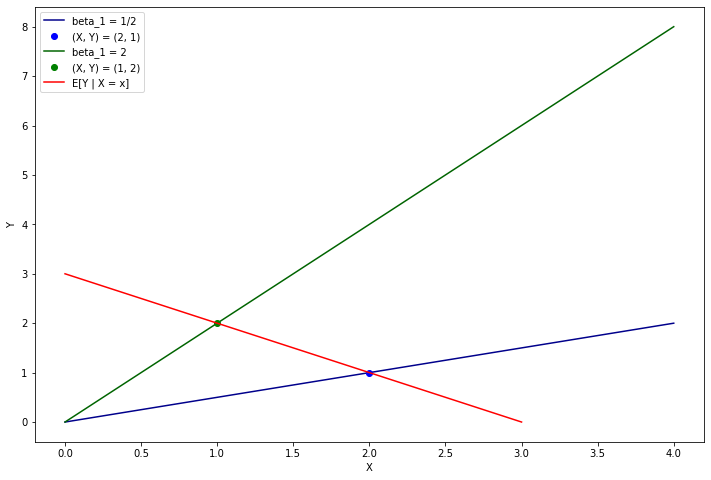
\includegraphics{Figure-19-01}
\end{figure}

Generally, what we want to do to make \(r(x) = \mathbb{E}(Y | X = x)\)
is to ensure the distribution generates points that have a lower \(X\)
for a larger \(Y\), by selecting a smaller value of \(X\) when \(Y\) is
larger.

Choose a joint probability distribution as
\(\mathbb{P}(\beta_{1}, x) = \mathbb{P}(\beta_{1}) \mathbb{P}(x | \beta_{1})\),
and  choose distribution of \(x | \beta_{1}\) as a discrete
probability mass function with all its mass on a single value:

\[
\mathbb{P}(x | \beta_{1}) = \begin{cases}
1 & \text{if } x + y = 1, \text{ where } y = \beta_{1} x\\
0 & \text{otherwise}
\end{cases}
\]

Now, by construction all points \((X, Y)\) lie on the line
\(X + Y = 1\), so \(\mathbb{E}(X + Y) = 1\) and
\(\mathbb{E}(Y | X = x) = 1 - x\), which is decreasing in \(x\).
